%======================================================================================
\chapter{Introdução} \label{cap:intro}
%======================================================================================

\section*{Introdução e Justificativa}

A reconstrucão 3D de cenas gerais a partir de múltiplos pontos de vista
usando-se câmeras convencionais, sem aquisição controlada, é um dos grandes
objetivos de pesquisa em visão computacional, ambicioso até mesmo para os dias
de hoje. Aplicações incluem a reconstrução de modelos 3D para uso em
videogames~\cite{ablan2007digital}, filmes~\cite{ablan2007digital},
arqueologia, arquitetura, modelagem 3D urbana (\eg, Google Streetview); técnicas
de \emph{match-moving} em cinematografia para fusão de conteúdo virtual e
filmagem real~\cite{dobbert2012matchmoving}, a organização de uma coleção de
fotografias com relação a uma cena (\eg, o sistema
\emph{Phototourism}~\cite{agarwal2010reconstructing} e a funcionalidade
\emph{Look Around} do Google Panoramio e Steet View), manipulação robótica, e a
metrologia a partir de câmeras na indústria automobilística e metal-mecânica.

Os desafios estão ligados às escolhas de grande escala de
representações adequadas e de técnicas que possam modelar simultaneamente com
materiais drasticamente diferentes (\eg, não-Lambertianos), modelos
geométricos (\eg, variedades curvilíneas gerais, descontinuidades, texturas,
deformações, em escalas diferentes), tipos de regiões (com ou sem textura),
condições de iluminação variadas, sombras, fortes diferenças de perspectivas,
desbalanceamento devido a excesso de detalhes em partes menos importantes,
número arbitrário de objetos e câmeras não-calibradas.

Mesmo que um sistema completo esteja fora do alcance da tecnologia atual,
um progresso significativo tem sido atingido nos últimos anos. Por um lado,
uma tecnologia operacional tem evoluído, mais recentemente para sistemas de grande
escala~\cite{agarwal2011building},
a partir do desenvolvimento da detecção robusta de
\emph{features}~\cite{mikolajczyk2002detection}, o
\emph{fitting}/ajuste robusto e seleção de correspondências baseados em \ransac, e o
desenvolvimento de métodos de geometria projetiva para calibrar duas ou três
imagens e progressivamente adicionar imagens e extrair estrutura 3D dessas
\emph{features} na forma de nuvens de pontos. Com o código fonte do sistema
Bundler~\cite{snavely2010bundler} liberado por Noah Snavely, e sua subsequente incorporação
ao sistema VisualSfM~\cite{wu2011visualsfm}, torna-se possível tentar utilizar este sistema para a
reconstrução de patrimônio cultural em larga escala, como um jardim de
esculturas. Um dos objetivos do presente trabalho é estudar até onde se pode
chegar com a aplicação de tais técnicas recentes à futura reconstrução completa do Jardim
do Nêgo, em Nova Friburgo, como parte de um projeto maior.

No paradigma usando-se apenas imagens convencionais -- denominado
\textbf{reconstrução estéreo multiocular passiva} --  a posição das câmeras são
estimadas a partir apenas de imagens, usando pontos de interesse; em seguida, uma
nuvem de pontos é reconstruída~\ref{fig:reconstrucaoEsparsaVisualSFM},\ref{fig:reconstrucaoEsparsaVisualSFM},\ref{fig:reconstrucaoEsparsaVisualSFM224}, \ref{fig:mvesfm}.
As câmeras podem então ser utilizadas para obter modelos mais detalhados de
reconstrução, como algoritmos de densificação~\cite{furukawa2007dense} e
interpolação~\cite{poisson} da nuvem de pontos, bem como demais algoritmos
densos de visão estéreo multi-perspectiva/multi-ocular, como os do grupo de
Michel Goesele~\cite{mve}, também com código disponível. Tais algoritmos, no
entanto, apresentam problemas, em particular a reconstrução suaviza partes
bem-delineadas do objeto, e pode conter buracos em áreas homogêneas. Pode-se,
portanto, utilizar no futuro a reconstrução 3D de curvas 
desenvolvida pelo grupo do prof.~Fabbri~\cite{Usumezbas:Fabbri:Kimia:ECCV16,Fabbri:Kimia:IJCV2016,Fabbri:Kimia:CVPR10,Fabbri:Giblin:Kimia:ECCV12}
para auxiliar na reconstrução mais bem-delinada nesses casos problemáticos, bem
como para ajudar no problema de escalabilidade quando a reconstrução 3D se torna
muito grande.  

Um segundo paradigma, denominado \textbf{reconstrução estéreo
multiocular ativa}, tem se tornado economicamente viável devido à indústria de videogames, e
consiste na utilização de sistemas que alteram o funcionamento de câmeras
convencionais, típicamente usando-se projetores infra-vermelho, \emph{laser} ou câmeras
ToF (\emph{Time of Flight}), como no caso dos dispositivos Kinect,
Figura~\ref{fig:kinect}.

\begin{figure} [!h]
	\centering
	%   \includegraphics[width=1.0\linewidth]{figs/3d-curve-sketch/system-diagram.eps}
	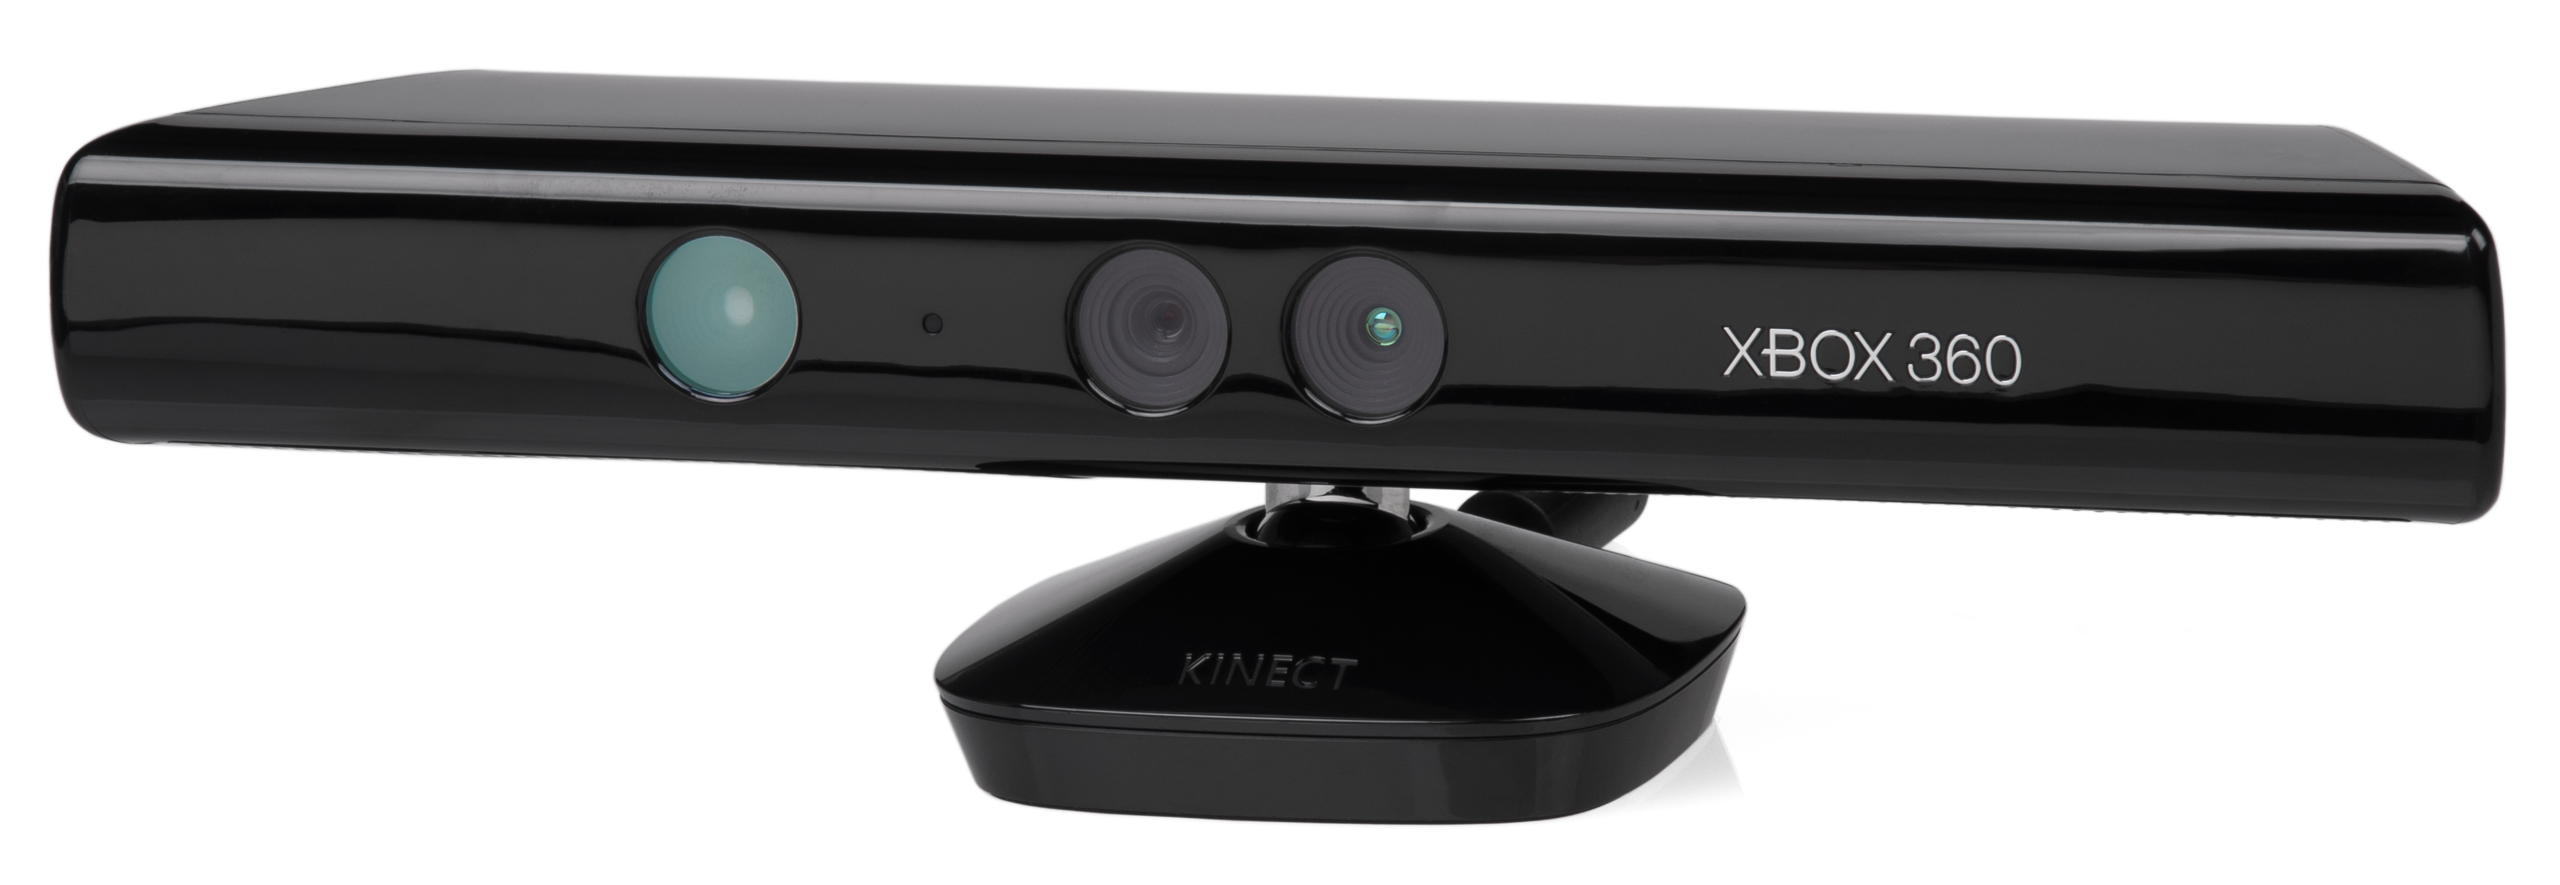
\includegraphics[width=0.45\linewidth]{figs/Xbox-360-Kinect-Standalone.png}(a)
	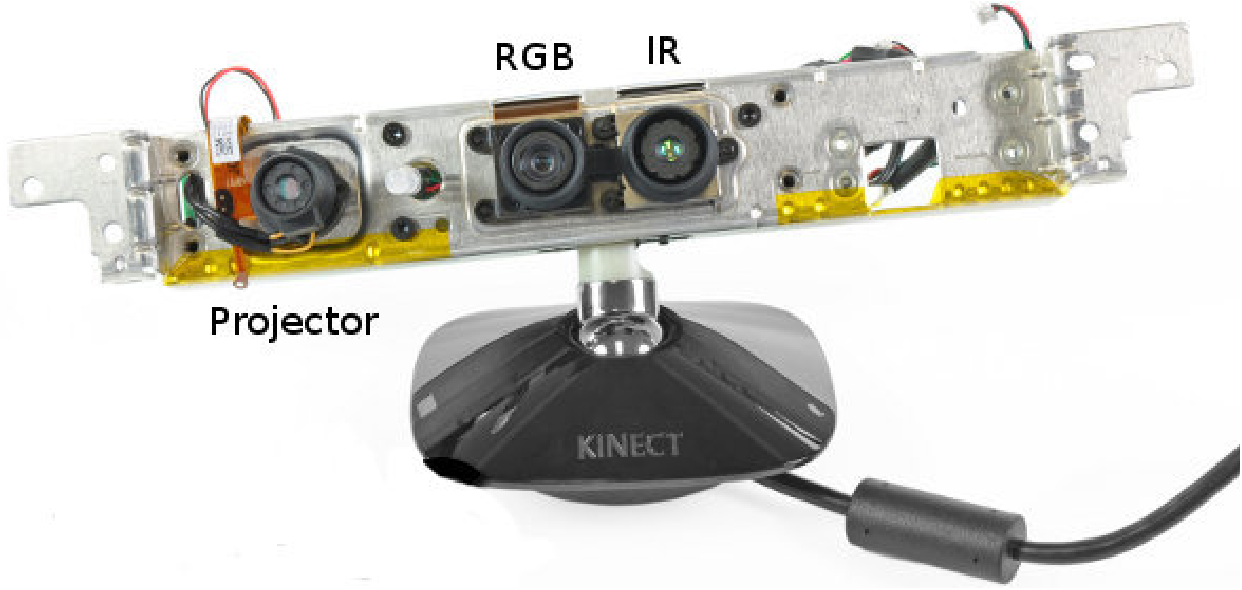
\includegraphics[width=0.45\linewidth]{figs/kinect-internals.pdf}(b)
 	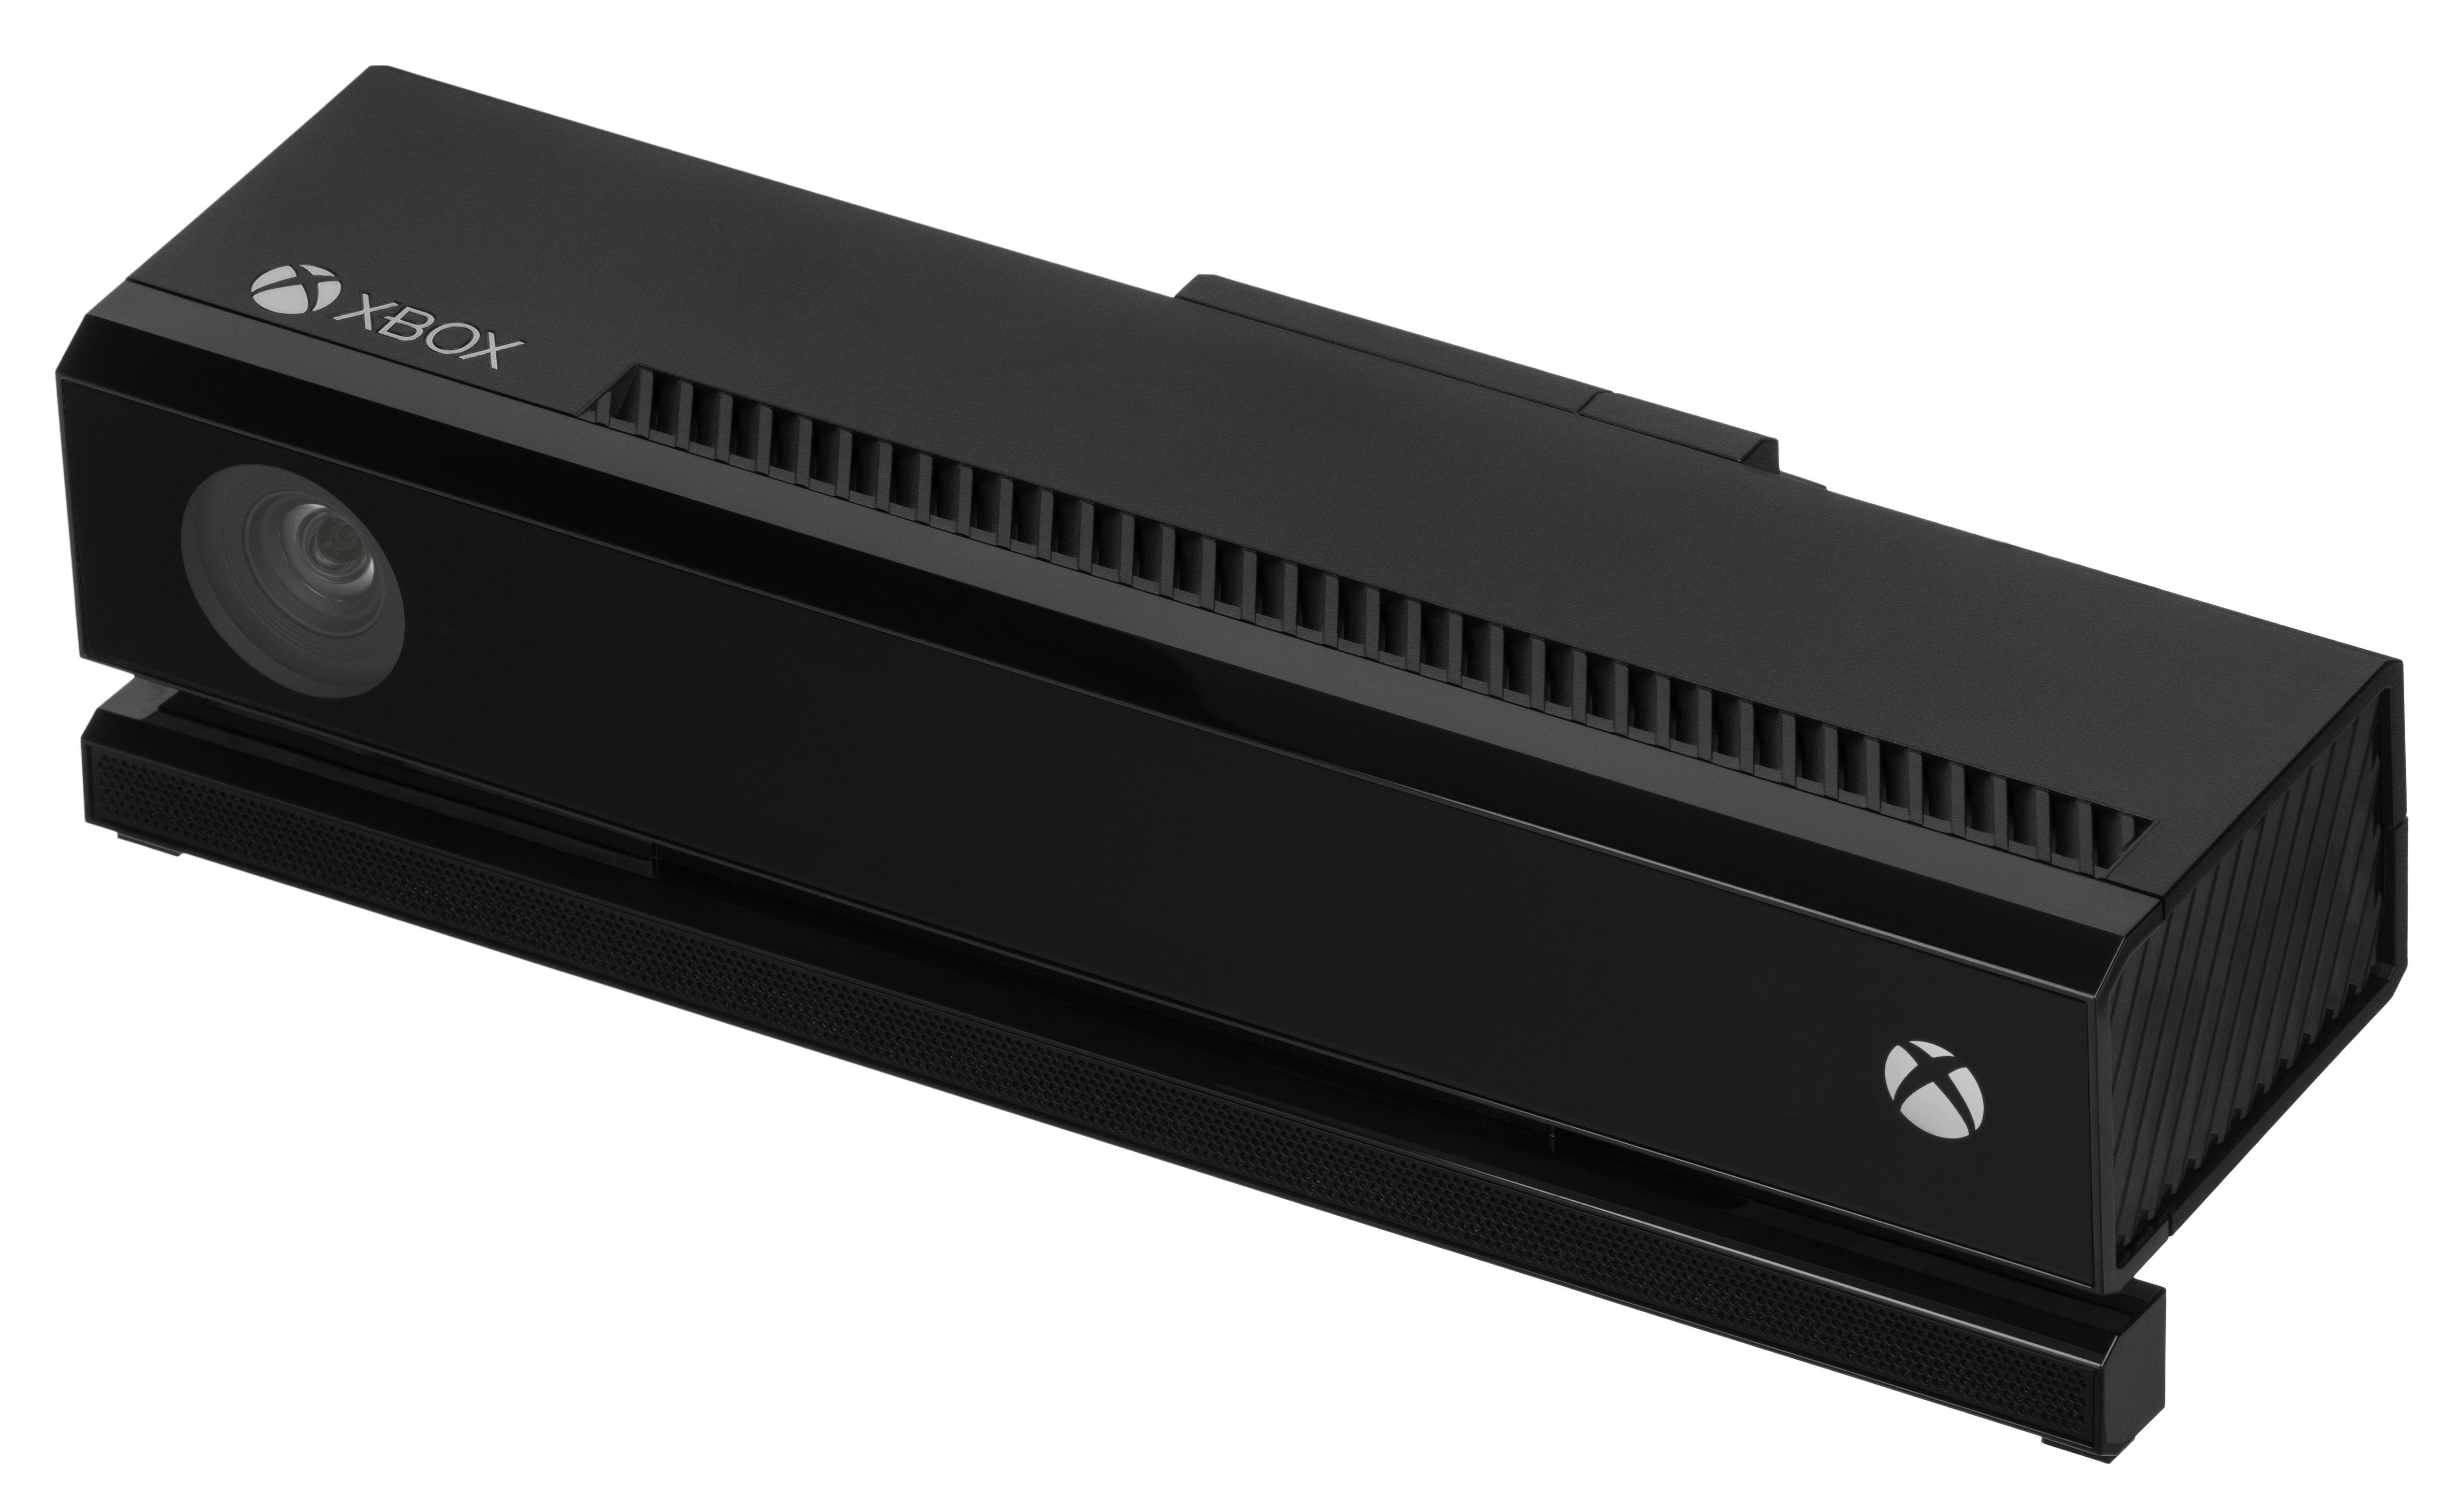
\includegraphics[width=0.45\linewidth]{figs/Xbox-One-Kinect.jpg}(c)
 	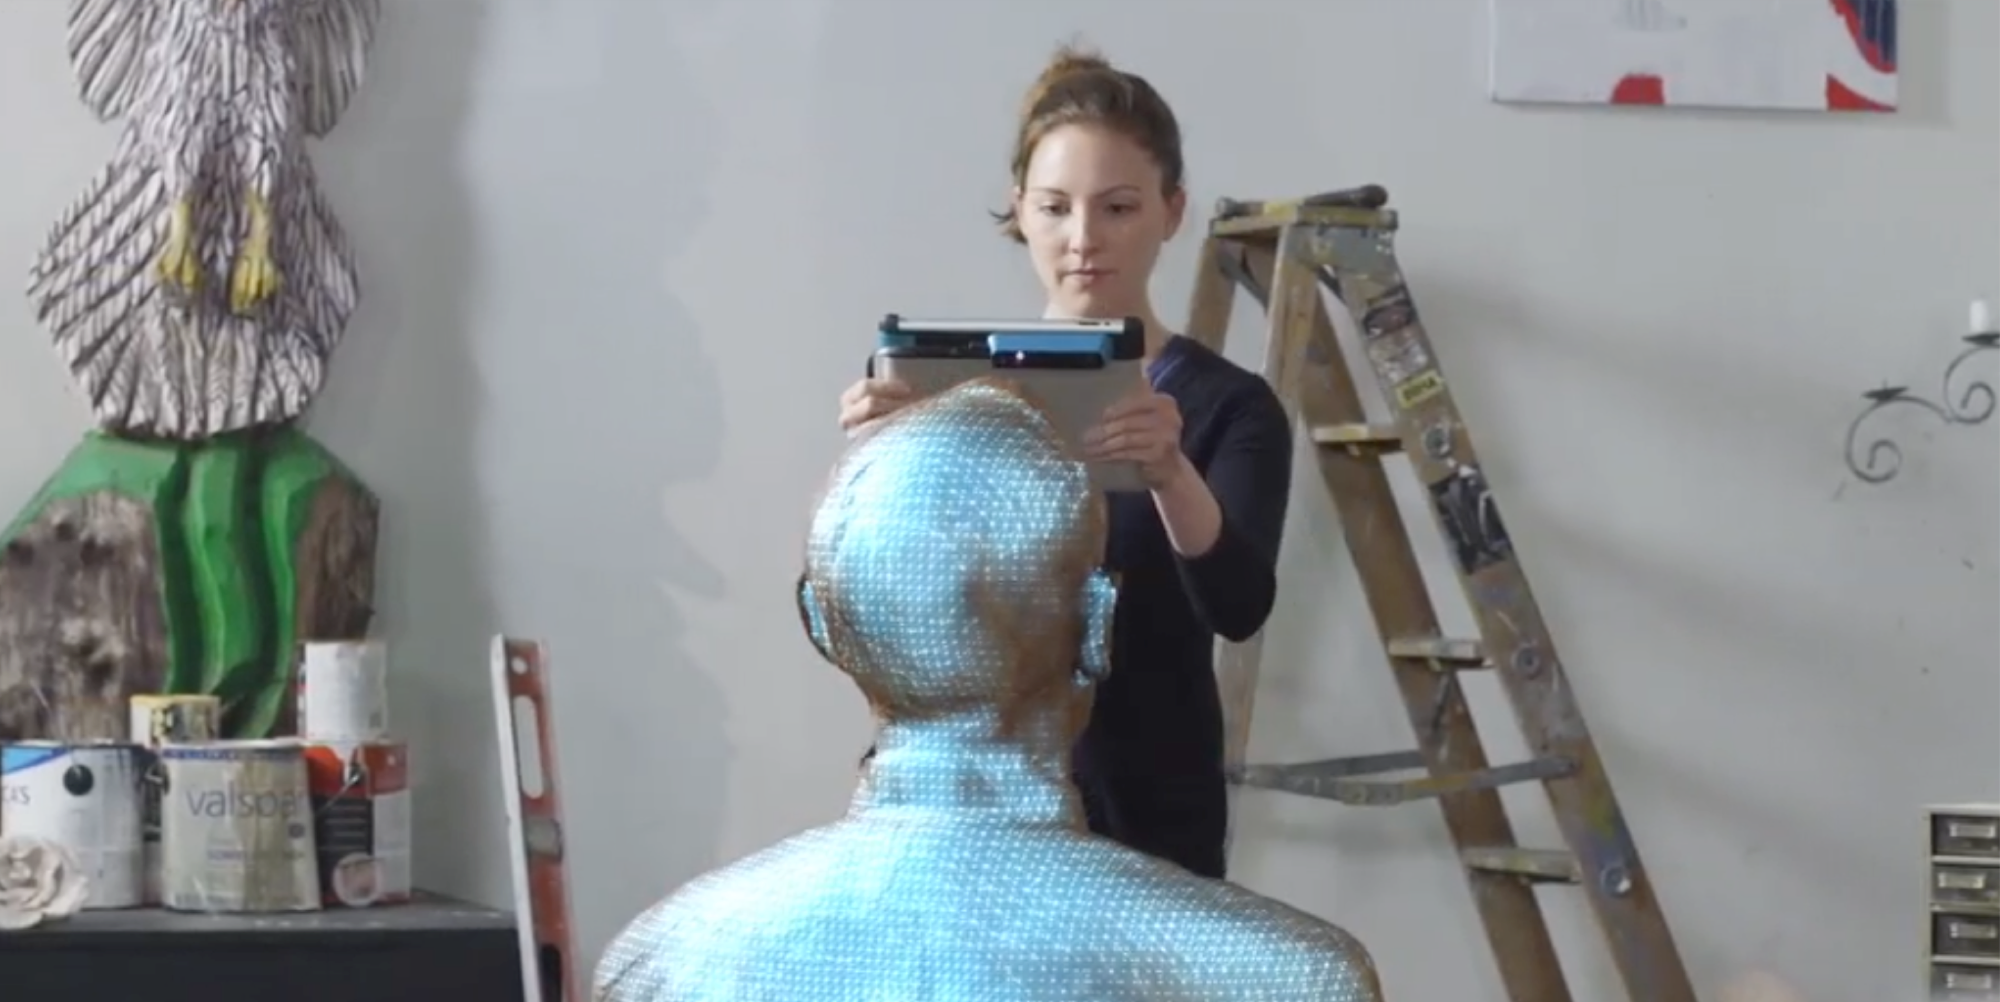
\includegraphics[width=0.45\linewidth]{figs/kinect-handheld1.png} (d)
	\caption{%
   Kinects de primeira geração (a) consistindo de câmeras e projetores
   infra-vermelho (b) e de segunda geração, consistindo de tecnologia ToF (c). 
   Ambos os kinects são largamente utilizados para escaneamento em tempo real, 
   formando a base de escaneadores manuais (d), porém nem sempre são úteis para 
   preservação detalhada de patrimônio. Um dos objetivos deste
   projeto é explorar os limites desta tecnologia.
	}\label{fig:kinect}
\end{figure}

A preservação de patrimônio tem sido realizada tradicionalmente com escaneadores
dedicados de alto custo, como no famoso projeto de escaneamento \emph{in situ} da escultura
David, chamado \emph{Digital Michaelangelo}~\cite{levoy2000digital},
Figura~\ref{fig:david}.  O projeto teve início em 1992 e tem como objetivo a
utilização de escaneadores a \emph{laser} de profundidade (\emph{Rangefinder Scanners}),
aliado a algoritmos que combinam diferentes profundidades e cores da imagem,
para realizar uma digitalização da parte externa e da superficie de forma
acurada da estátua de David. Note-se, porém, que esse método pode ser utilizado em diferentes
objetos no mundo real, como partes de máquinas, artefatos culturais e na
indústria de video games, por exemplo.  Para as partes mais detalhadas, foi
utilizado um escaneador de menor escala que faz uma pequena triangulação com
laser de profundidade.

Mais recentemente, pode-se considerar tecnologias mais acessíveis, similares às
de altíssimo custo do projeto Digital Michaelangelo e popularizadas na última
década pela indústria de entretenimento, notadamente pelo projeto
Natal/Kinect~\cite{smisek20133d,wang2015research}. A reconstrução usando-se Kinect (de
primeira ou segunda geração) usando software atual de super-resolução, é
inferior à de um sistema a \emph{laser} de alta qualidade, sendo, porém de baixo custo
e muito mais versátil devido ao sistema de aquisição manual e a software
amplamente utilizado e desenvolvido~\cite{wang2015research},
Figura~\ref{fig:rec3d:comparacao}.

% Seria de grande interesse explorar os dois paradigmas supracitados
% para avaliar as possibilidades disponíveis no estado da arte de reconstrução 3D
% para o escaneamento de baixo custo para a preservação de Patrimônio. O que se
% pode atingir com apenas uma filmagem de esculturas realizada por um smartphone,
% sem calibração prévia e \emph{in situ}, ou seja, sem ambiente controlado?  Como
% esta recontrução se compara nos dias de hoje com a reconstrução realizada por um
% escaneador padrão baseado em Kinect?

\begin{figure}[!h]
	\centering
	%   \includegraphics[width=1.0\linewidth]{figs/3d-curve-sketch/system-diagram.eps}
	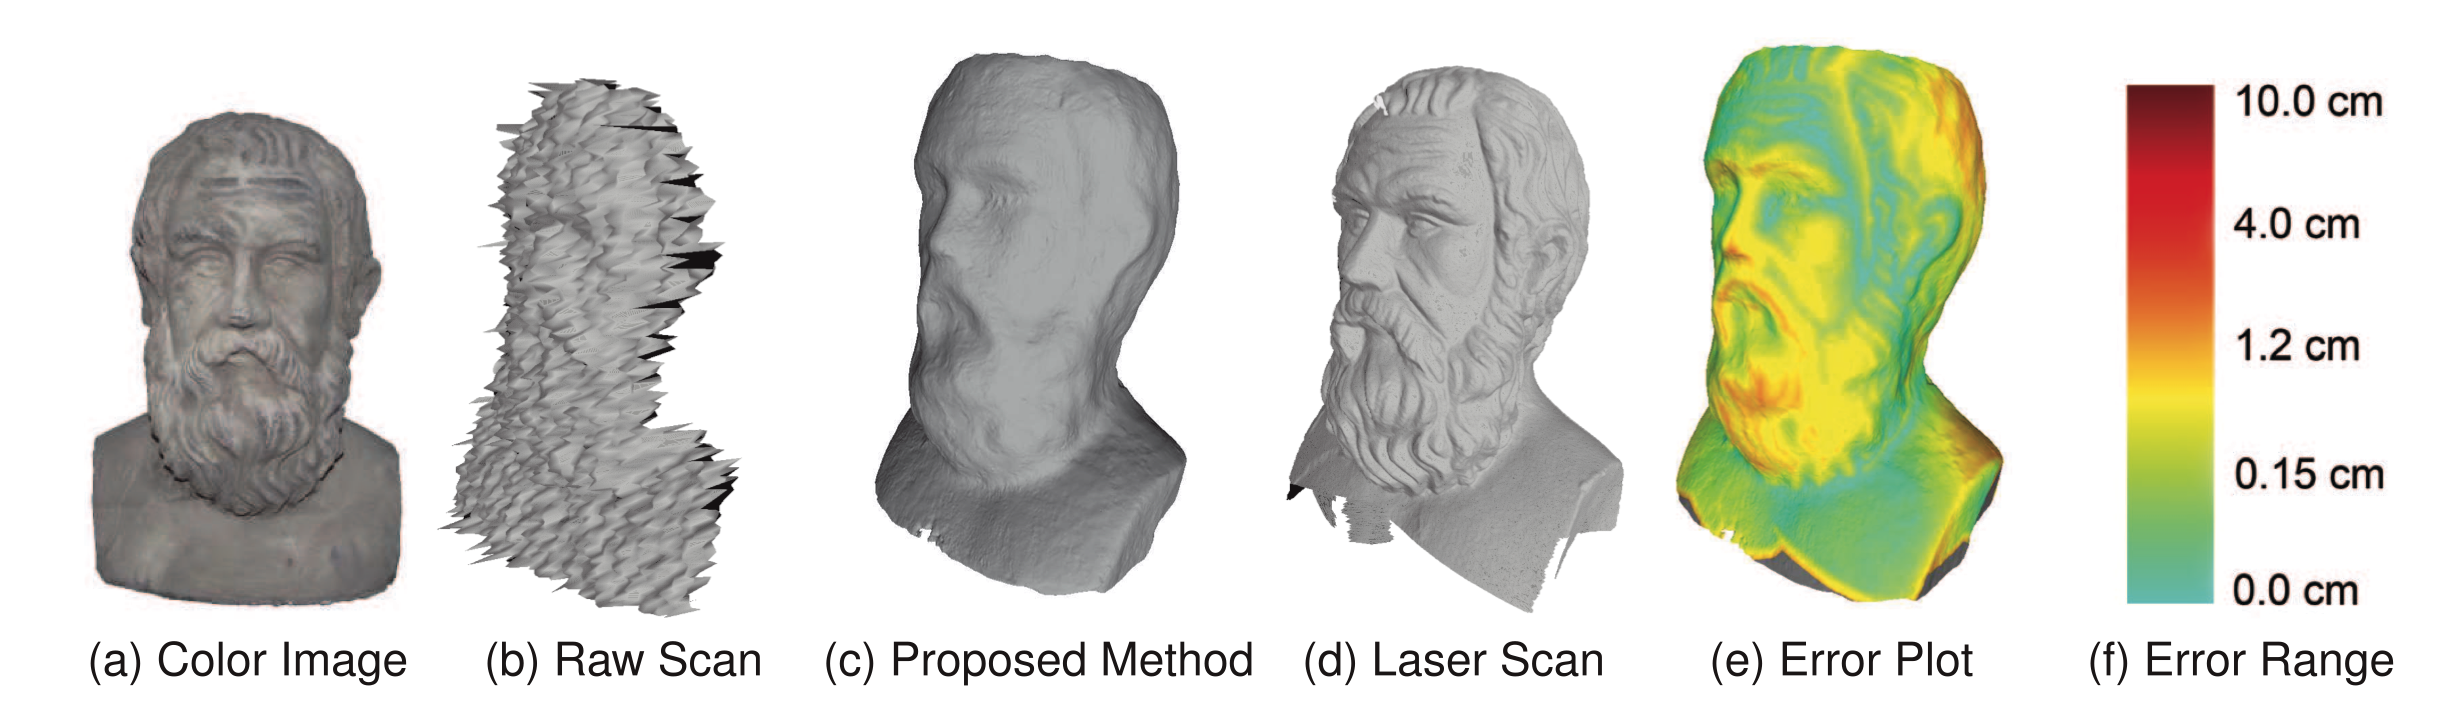
\includegraphics[width=1\linewidth]{figs/kinect-vs-usual.png}
	\caption{%
    A reconstrução usando-se Kinect (de primeira ou segunda geração) usando
    software atual de super-resolução (c) fornece precisão similar a um sistema estéreo de média
    resolução, inferior um sistema a \emph{laser} de alta qualidade (d) porém de baixo custo e
    muito mais versátil devido ao sistema de aquisição manual e a software
    amplamente utilizado e
    desenvolvido~\cite{wang2015research}.
	}\label{fig:rec3d:comparacao}
\end{figure}

\begin{figure}[!h]

\centering

\subfloat[]{\label{fig:davida}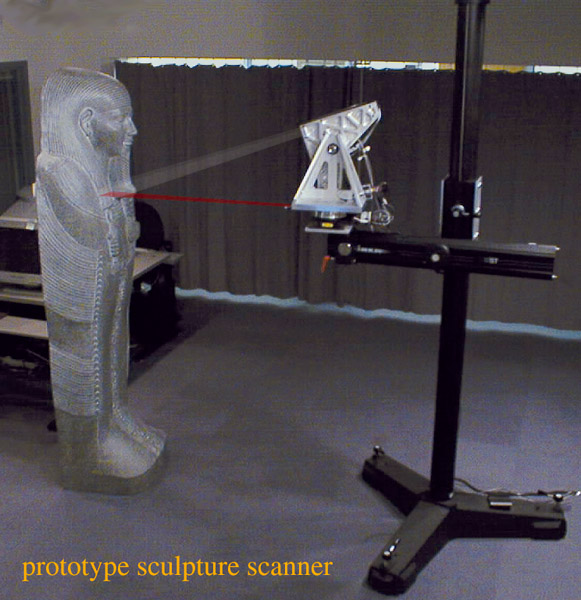
\includegraphics[width=0.18\linewidth]{figs/Proto+Inka+Egypt_light-s.jpg}}
% \vspace{2ex}
\subfloat[]{\label{fig:davidb}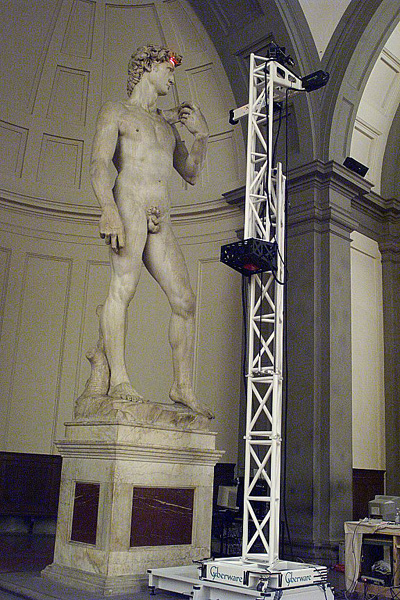
\includegraphics[width=0.18\linewidth]{figs/gantry-with-david-s.jpg}}
\subfloat[]{\label{fig:davidc}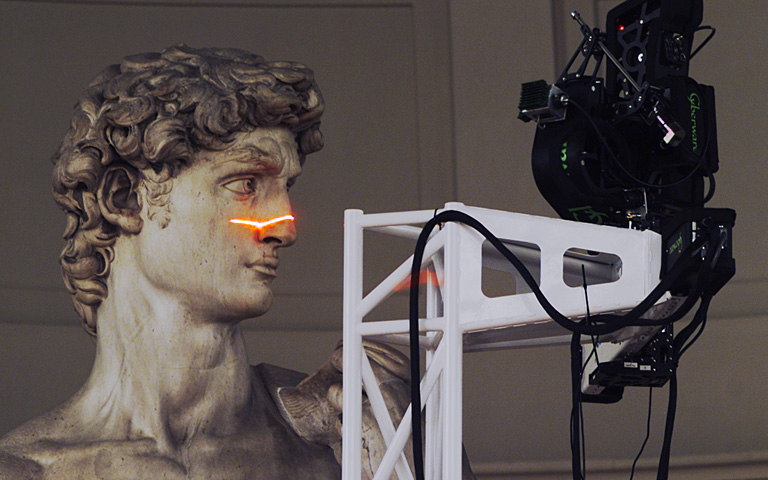
\includegraphics[width=0.18\linewidth]{figs/scanner-head-and-david-head-s.jpg}}
% \vspace{2ex}
\subfloat[]{\label{fig:davidd}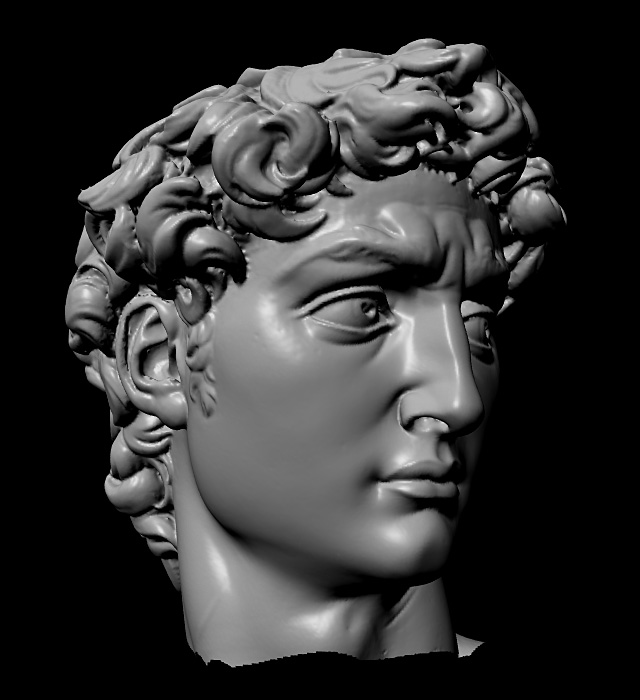
\includegraphics[width=0.18\linewidth]{figs/david-classic-leftlight-s.jpg}}
\caption{%
   Protótipo do escaneador a \emph{laser} de triangulação. O objeto a ser escaneado é uma réplica em tamanho real
   de um sarcófago egípcio (a). O escaneador foi reconfigurado para escanear objetos maiores, pois 
   a escultura possui 517 centímetros (b), o da cabeça também sofreu uma reconfiguração, este escaneador gira em 90 graus, 
   que faz o \emph{laser} rotacionar, da posição horizontal para a vertical e também roda em torno da cabeça como um todo (c).
   Para a reconstrução, o primeiro passo foi alinhar cerca de 100 scans em
   diversas posições, após isso, utilizado um 
   alinhamento automatico em pares dos scans, utilizando um algoritmo modificado de iteracoes de pontos próximos 
   (ICP - \emph {Iterated-Closest-Points}). Após isso, faz-se um processo de relaxação global a fim de minimizar erros 
   de alinhamento por toda a estátua. Depois de alinhados, usa-se o algoritmo de profundidade volumétrica de 
   processamento de imagens (VRIP - \emph {Volumetric Range Image Processing} -
   de Brian Curless) (d)~\cite{levoy2000digital}}.
  \label{fig:david}
\end{figure}

\subsection*{O Jardim do Nêgo, Nova Friburgo}
No caso de Nova Friburgo, há a necessidade redobrada de preservação de
patrimônio a céu aberto, em especial devido às chuvas e deslizamentos inerentes à região.  O
Jardim do Nêgo consiste em grandes esculturas em encostas, cobertas por um tapete de
vegetação, as quais desfrutam de grande reconhecimento regional e internacional~\cite{JardimDoNego:TheGuardian},
Figura~\ref{fig:esculturas}.

\begin{figure} [!h]
	\centering
	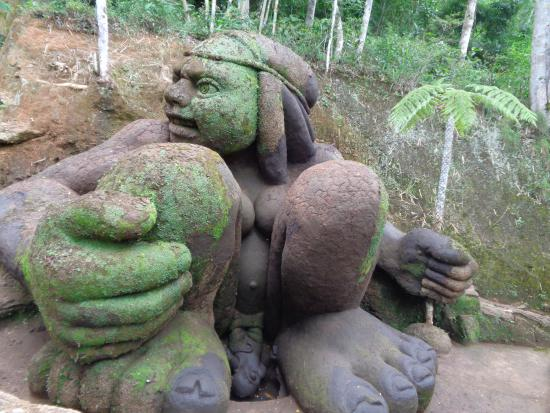
\includegraphics[width=0.3\linewidth]{figs/jardim-do-nego.jpg}
	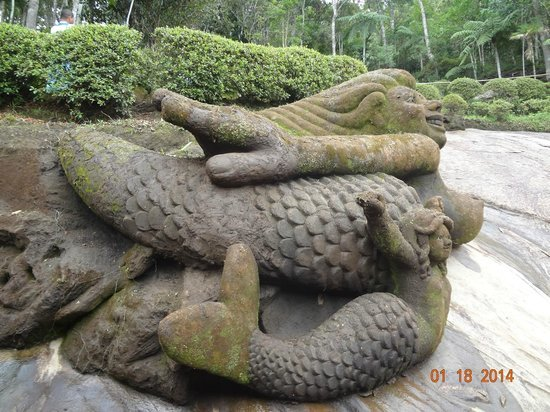
\includegraphics[width=0.3\linewidth]{figs/jardim-do-nego22.jpg}
	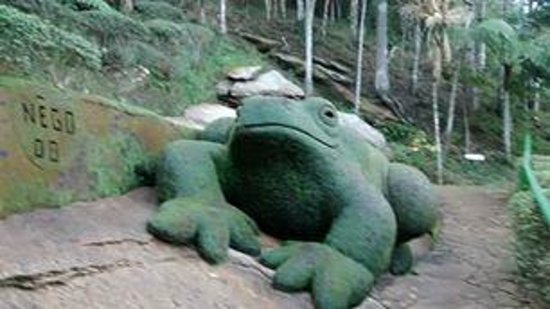
\includegraphics[width=0.35\linewidth]{figs/jardim-do-nego32.jpg}
	\caption{Algumas esculturas do Jardim do Nêgo~\cite{JardimDoNego:TheGuardian}}\label{fig:esculturas}
\end{figure}


% \begin{figure} [!h]
% 	\centering
% 	%   \includegraphics[width=1.0\linewidth]{figs/3d-curve-sketch/system-diagram.eps}
% 	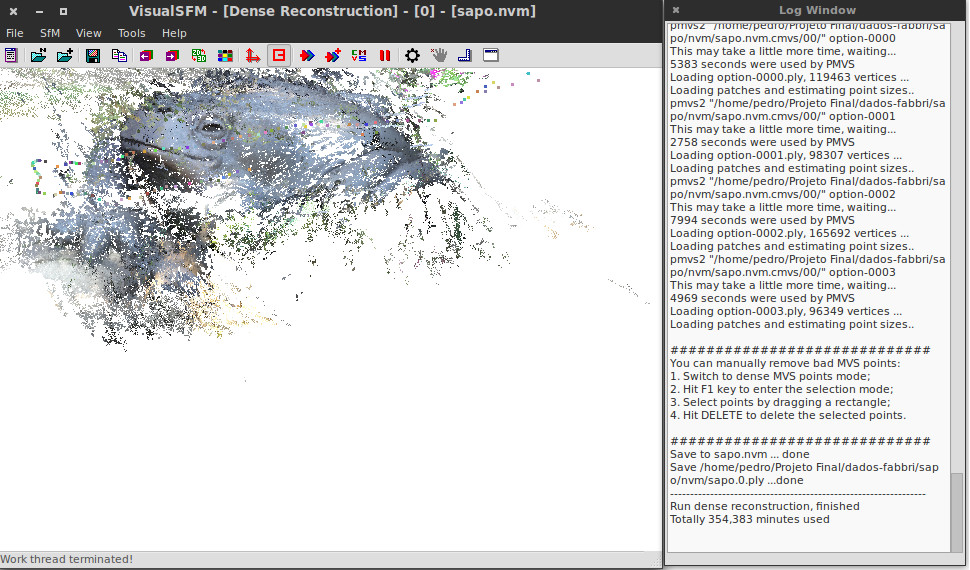
\includegraphics[width=1\linewidth]{figs/rec3d.jpg}
% %	\includegraphics[width=0.95\linewidth]{figs/rec3d-curves-pmvs.pdf}
% 	\label{fig:rec3d}
% 	\caption{A reconstrução usando-se apenas imagens, sem controle de aquisição, 
% 	   como em um vídeo de um smartphone filmado em torno do objeto, fornece uma
% 	   nuvem de pontos, que pode ser
% 	   densificada~\cite{snavely2010bundler,wu2011visualsfm,furukawa2007dense,mve}, ou
% 	   atribuída de
% 	   curvas~\cite{Usumezbas:Fabbri:Kimia:ECCV16,Fabbri:Kimia:IJCV2016,Fabbri:Kimia:CVPR10,Fabbri:Giblin:Kimia:ECCV12}, de forma a preservar a resolução
% 	   em áreas de alto conteúdo informativo. Tais representações estão sendo
% 	   atualmente unificadas na pesquisa da área. Este projeto propõe explorar os
% 	   limites da reconstrução 3D usando-se apenas imagens, no contexto de
% 	   preservação de patrimônio.}
% \end{figure}


Idealizado e criado por Geraldo Simplicio (Nêgo), artista cearense que mora no
local a mais de 30 anos, e que ganhou notoriedade por suas esculturas de barro,
com traços singulares e técnicas únicas. Hoje, trabalha para reconstruir o
Jardim após a tragédia de 2011 na região serrana, onde algumas estruturas foram
destruídas. Portanto, com o consentimento do Nêgo, surgiu a motivação desta
pesquisa: além de explorar métodos de reconstrução, também tem o objetivo de
ajudar a criar sistemas completos para eternizar um patrimônio que é reconhecido
no mundo todo.

A preservação das esculturas do Jardim do Nêgo se mostra um desafio à pesquisa em
recontrução 3D, pois apresentam curvas bem delineadas, que são 
representadas de maneira suavizada e empobrecida por métodos convencionais.
Algumas esculturas apresentam pouca textura, com apenas um leve padrão de musgo.
Seria de grande interesse avaliar o potencial de técnicas atuais de
reconstrução 3D geral que não exigem controle preciso de aquisição, as quais têm seu código fonte
disponível na internet.

\newpage

\section{Objetivos}\label{sec:objetivos}

Pretende-se, ao longo deste projeto, ganhar experiência com técnicas
modernas de reconstrução 3D fotogramétrica, no contexto de uma aplicação
bem-definida de preservação de patrimônio. 
% A entrada do sistema deverá ser um
% conjunto de vídeos realizados por câmeras de baixo custo, ou um conjunto de
% escaneamentos realizados por escaneadores à mão de baixo custo baseados em Kinect.

O objetivo concreto é explorar as tecnologias supracitadas para
desenvolver um esquema de escaneamento de patrimônio usando software aberto, câmeras e
escaneadores de baixo custo, representando o estado da arte em reconstrução 3D sem
restrições de aquisição. Perguntas fundamentais a serem respondidas são: que
nível de detalhe, facilidade e precisão se pode obter usando-se apenas imagens e software
aberto? É possível utilizar escaneadores de baixo custo baseados em Kinect com
melhorias significativas em termos de qualidade, conveniência ou tempo de
processamento?  Quais são as restrições desses sistemas? Seria útil, na prática,
uma reconstrução de curvas para auxiliar na reconstrução de nuvem de pontos e de
superfícies densas? Onde o estado da arte deve ser avançado de forma a permitir
uma solução mais conveniente e completa para a preservação de patrimônio?

O principal objetivo em termos de pesquisa científica será comparar as
diferentes abordagens do estado da arte disponíveis para reconstrução 3D e
explicitar suas limitações práticas.

\section*{Organização deste manuscrito}

Este trabalho foi estruturado da seguinte maneira: Introduzimos
métodos baseados em reconstrução a \emph{laser} no Capítulo~\ref{cap:laser},
apresentando, de uma maneira mais técnica, o projeto \emph{Digital
Michelangelo} na Seção~\ref{sec:David}, que foi um dos pioneiros na técnica de
conservação de acervos culturais. No próximo Capítulo~\ref{cap:kinect},
discutimos o uso do Kinect, da Microsoft, no que tange à calibração do sistema
para o uso em tecnologias \emph{Structure from Motion}.  Adiante, no
Capítulo~\ref{cap:pontosdeinteresse}, abordaremos o tema central do trabalho:
técnicas de reconstrução baseadas em fotogrametria, com o emprego de dois
softwares, o MVE~\ref{sec:mve} e o VisualSfM~\ref{sec:visualsfm} e seus
respectivos funcionamentos. Ao final, apresentamos experimentos e conclusões
do trabalho, bem como sugestões para implementações e trabalhos futuros.

% O trabalho foi estruturado da seguinte maneira: previamente introduzimos os métodos baseados em pontos de interesse no Capítulo~\ref{sec:pontosdeinteresse}, destacando suas funcionalidades. No Capítulo~\ref{sec:denserecon} discutimos e aprofundamos o  funcionamento de cada algoritmo de reconstrução densa empregados, apresentando e debatendo, comparativamente, pontos à favor e contra; O Capítulo~\ref{sec:kinect} é apresentada a técnica de reconstrução utilizada nos  {\it Kinects}, da Microsoft; Com isso, temos o  Capítulo~\ref{sec:visualsfm}, que é dedicado à ferramenta gráfica utilizada para a obtenção dos resultados (VisualSfM) dos algoritmos de reconstrução densa utilizados. Finalmente, apresentamos os resultados e conclusões do trabalho, bem como sugestões para implementações e trabalhos futuros.
%Este trabalho está organizado da seguinte forma: discutimos as técnicas de
%extração de curva sem aprendizagem de máquina supervisionada no
%Capítulo~\ref{sec:cfrag:extraction}. No Capítulo~\ref{sec:learning:chapter},
%discutimos maneiras pelas quais essas técnicas podem ser melhoradas
%usando dados de treinamento anotados por humanos como entrada para uma
%aprendizagem de máquina geométrica de topologia e semântica de fragmentos de
%curva. A maior parte deste material é
%de~\cite{Guo:etal:CVPR14,Guo:etal:PAMI2017:submitted,Tamrakar:PHD:2008}, com esclarecimentos
%substanciais e comentários sobre as questões relativas aos nossos objetivos
%específicos. No Capítulo~\ref{sec:generic:datasets}, apresentamos o processo de
%captura de dados confiáveis (\emph{ground-truth}), comparando os conjuntos de dados anteriores com o problema proposto
%neste trabalho para a água. Nos capítulos restantes, apresentamos e discutimos
%nossos resultados para vários vídeos em tanques de água. Partes deste trabalho
%foram apresentadas em~\cite{Fabbri:WaterWaves2016,Fabbri:WaterWaves2017,Souza:Fabbri:WaterWaves2017}.

%======================================================================================
